% !TeX program = xelatex
\documentclass[a4paper,10pt]{article}

% ============================================================================
% កញ្ចប់បណ្ណាល័យ (Packages) – តាមលំនាំ NGS Preah Krasang (ls_plan.tex)
% បរិបទ៖ គ្មានស្លាយ LCD និងគ្មានម៉ាស៊ីនគិតលេខ — ប្រើសន្លឹកកិច្ចការសិស្ស (ស-ខ្មៅ) និងក្ដារខៀនជាគោល
% ============================================================================
\usepackage[a4paper, left=0.95cm, right=0.95cm, top=0.85cm, bottom=0.92cm, footskip=0.52cm]{geometry}
\usepackage{amsmath, amssymb}
\usepackage{unicode-math}
\usepackage{fontspec}
\usepackage{array, longtable, multirow, colortbl}
\usepackage[table]{xcolor}
\usepackage{enumitem}
\usepackage{pifont}
\usepackage{fancyhdr}
\usepackage{tikz}
\usetikzlibrary{calc, arrows.meta, angles, quotes, decorations.markings, decorations.pathreplacing, patterns, babel}

\makeatletter
\let\@expl@@@mark@update@singlecol@structures@@\relax
\makeatother

\providecommand{\NGSFindFonts}{%
  \IfFileExists{C:/Windows/Fonts/cambria.ttc}{%
    \def\NGSSysPath{C:/Windows/Fonts/}%
    \def\NGSUserPath{C:/Users/KIT/AppData/Local/Microsoft/Windows/Fonts/}%
  }{%
    \IfFileExists{./fonts/KhmerOSsiemreap.ttf}{\def\NGSSysPath{./fonts/}\def\NGSUserPath{./fonts/}}{%
    \IfFileExists{../fonts/KhmerOSsiemreap.ttf}{\def\NGSSysPath{../fonts/}\def\NGSUserPath{../fonts/}}{%
    \IfFileExists{../../fonts/KhmerOSsiemreap.ttf}{\def\NGSSysPath{../../fonts/}\def\NGSUserPath{../../fonts/}}{%
    \IfFileExists{../../../fonts/KhmerOSsiemreap.ttf}{\def\NGSSysPath{../../../fonts/}\def\NGSUserPath{../../../fonts/}}{%
    \IfFileExists{../../../../fonts/KhmerOSsiemreap.ttf}{\def\NGSSysPath{../../../../fonts/}\def\NGSUserPath{../../../../fonts/}}{%
    \IfFileExists{../../../../../fonts/KhmerOSsiemreap.ttf}{\def\NGSSysPath{../../../../../fonts/}\def\NGSUserPath{../../../../../fonts/}}{%
    \IfFileExists{../../../../../../fonts/KhmerOSsiemreap.ttf}{\def\NGSSysPath{../../../../../../fonts/}\def\NGSUserPath{../../../../../../fonts/}}{%
      \def\NGSSysPath{../../../../../../../fonts/}\def\NGSUserPath{../../../../../../../fonts/}%
    }}}}}}}%
  }%
}
\NGSFindFonts

\setmathfont[Path={\NGSSysPath}, FontIndex=1, Scale=1.02]{cambria.ttc}
\defaultfontfeatures{Ligatures=TeX}

\setmainfont[
  Path={\NGSUserPath}, Extension=.ttf, Script=Khmer,
  BoldFont={KhmerOSsiemreap}, BoldFeatures={FakeBold=1.8},
  ItalicFont={KhmerOSsiemreap}, ItalicFeatures={FakeSlant=0.25},
  BoldItalicFont={KhmerOSsiemreap}, BoldItalicFeatures={FakeBold=1.8, FakeSlant=0.25}
]{KhmerOSsiemreap}

\newfontfamily\muol[Path={\NGSUserPath}, Extension=.ttf, Script=Khmer]{KhmerOSmuollight}
\newfontfamily\TimesEn[Path={\NGSSysPath}, Extension=.ttf, Scale=1.00, BoldFont={timesbd}, ItalicFont={timesi}, BoldItalicFont={timesbi}]{times}
\newfontfamily\NagaBold[Path={\NGSUserPath}, Extension=.ttf]{AKbalthom Naga Bold}
\newfontfamily\CalibriFont[Path={\NGSSysPath}, Extension=.ttf]{calibri}
\newfontfamily\Tacteing[Path={\NGSUserPath}]{TACTENG.TTF}
\newfontfamily\CourierBullet[Path={\NGSSysPath}, Extension=.ttf]{cour}
\newcommand{\wcirc}{{\CourierBullet\fontsize{9.5pt}{11pt}\selectfont o}}

\XeTeXlinebreaklocale "km"
\XeTeXlinebreakskip = 0pt plus 1pt minus 0.1pt

\definecolor{stepgray}{HTML}{D9D9D9}
\definecolor{headgray}{HTML}{F2F2F2}
\definecolor{boxgray}{HTML}{D9D9D9}
\definecolor{darkred}{HTML}{C00000}
\definecolor{red5e}{HTML}{FF0000}

\pagestyle{fancy}
\fancyhf{}
\renewcommand{\headrulewidth}{0pt}
\fancyfoot[R]{\CalibriFont\fontsize{11pt}{13pt}\selectfont\thepage}

\setlength{\parindent}{0pt}
\setlength{\parskip}{0pt}
\setlength{\tabcolsep}{3.8pt}

\newcolumntype{L}[1]{>{\raggedright\arraybackslash}p{#1}}
\newcolumntype{C}[1]{>{\centering\arraybackslash}p{#1}}

\newcommand{\en}[1]{{\TimesEn #1}}
\newcommand{\enbf}[1]{{\TimesEn\textbf{#1}}}
\newcommand{\unit}[1]{\,\text{\en{#1}}}
\newcommand{\fiveE}[1]{{\NagaBold\fontsize{9.5pt}{13pt}\selectfont\textcolor{red5e}{#1}}}
\newcommand{\timenote}[1]{\textcolor{darkred}{\textit{#1}}}
\newcommand{\graybox}[1]{\colorbox{boxgray}{\strut\hspace{2pt}#1\hspace{2pt}}}
\newcommand{\cnum}[1]{{\fontsize{10.5pt}{12pt}\selectfont\ding{\numexpr181+#1\relax}}\hspace{0.15em}}
\newcommand{\cfig}[1]{\par\vspace{3pt}{\centering #1\par}\vspace{3pt}}
\newcommand{\stepheader}[1]{\multicolumn{3}{|c|}{\cellcolor{stepgray}\muol #1} \\* \noalign{\hrule height 0.4pt}}
\newcommand{\khmflourish}{{\Tacteing\fontsize{36pt}{14pt}\selectfont\raisebox{-5pt}{3}}}

% ============================================================================
% ម៉ាក្រូគូសរូប TikZ ស-ខ្មៅ ១០០% សម្រាប់មេរៀន ៦ ចំណោទ និងសំយោគមេរៀនទី១ (RAT_PROB)
% ============================================================================

% ១. E1 Engage: គូប្រភាគអច្ឆរិយៈ 13/4 + 13/9 = 13/4 x 13/9 (លំហាត់ #11 ទំ.១២)
\newcommand{\figEngageRATPROB}{%
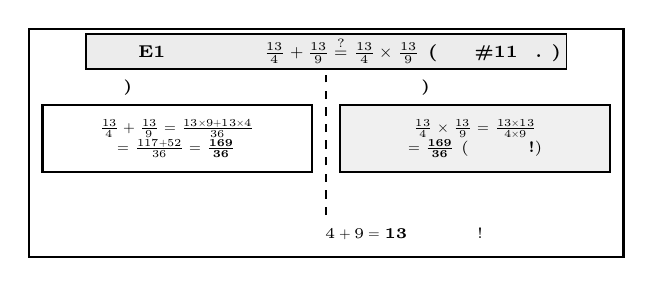
\begin{tikzpicture}[x=0.95cm, y=0.92cm, every node/.style={font=\scriptsize, text=black}]
  \draw[black, line width=0.95pt] (0,0) rectangle (7.95,3.15);
  \node[fill=gray!15, draw=black, line width=0.6pt, inner sep=2pt, font=\fontsize{6.2pt}{7.9pt}\selectfont\bfseries] at (3.975,2.84) {បេសកកម្ម \en{E1}៖ គូប្រភាគអច្ឆរិយៈ $\frac{13}{4}+\frac{13}{9} \stackrel{?}{=} \frac{13}{4}\times\frac{13}{9}$ (លំហាត់ \#11 ទំ.១២)};

  \draw[black, dashed, line width=0.65pt] (3.975,0.58) -- (3.975,2.52);

  \node[font=\fontsize{5.6pt}{7.2pt}\selectfont\bfseries] at (1.98,2.34) {១) គណនាផលបូកប្រភាគទាំងពីរ};
  \draw[black, line width=0.8pt] (0.18,1.18) rectangle (3.78,2.10);
  \node[align=center, font=\fontsize{5.5pt}{7.1pt}\selectfont] at (1.98,1.64) {$\frac{13}{4} + \frac{13}{9} = \frac{13\times 9 + 13\times 4}{36}$\\$= \frac{117 + 52}{36} = \mathbf{\frac{169}{36}}$};

  \node[font=\fontsize{5.6pt}{7.2pt}\selectfont\bfseries] at (5.96,2.34) {២) គណនាផលគុណប្រភាគទាំងពីរ};
  \draw[black, line width=0.8pt, fill=gray!12] (4.16,1.18) rectangle (7.77,2.10);
  \node[align=center, font=\fontsize{5.5pt}{7.1pt}\selectfont] at (5.965,1.64) {$\frac{13}{4} \times \frac{13}{9} = \frac{13\times 13}{4\times 9}$\\$= \mathbf{\frac{169}{36}}$ (\textbf{ស្មើគ្នាបេះបិទ!})};

  \node[font=\fontsize{5.4pt}{6.9pt}\selectfont] at (3.975,0.32) {\textbf{អាថ៌កំបាំងពីជគណិត៖} ព្រោះផលបូកភាគបែង $4 + 9 = \mathbf{13}$ ស្មើនឹងភាគយករួម!};
\end{tikzpicture}}

% ២. E2 POE 1 & POE 2: ប្លង់ចតុកោណកែង (ទំ.១០–១១) និងដ្យាក្រាមផ្លិតប្រាក់សន្សំ (#14 ទំ.១២)
\newcommand{\figModelsRATPROB}{%
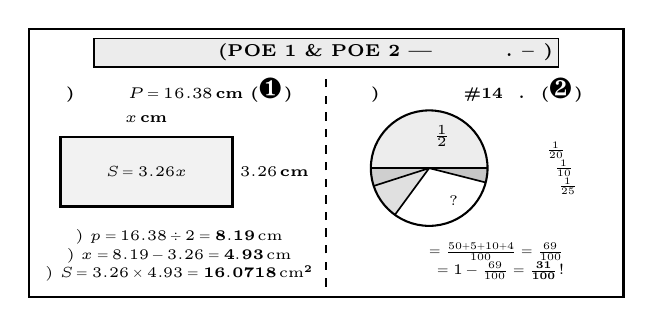
\begin{tikzpicture}[x=0.95cm, y=0.94cm, every node/.style={font=\scriptsize, text=black}]
  \draw[black, line width=0.95pt] (0,0) rectangle (7.95,3.62);
  \node[fill=gray!15, draw=black, line width=0.6pt, inner sep=2pt, font=\fontsize{6.2pt}{7.9pt}\selectfont\bfseries] at (3.975,3.30) {គំនូសប្លង់ដោះស្រាយចំណោទ \en{(POE 1 \& POE 2} — សៀវភៅពុម្ព ទំ.១០–១២)};

  \draw[black, dashed, line width=0.65pt] (3.975,0.14) -- (3.975,2.98);

  % Left: Rectangle P=16.38cm, width=3.26cm (ទំ.១០–១១)
  \node[font=\fontsize{5.6pt}{7.2pt}\selectfont\bfseries] at (1.98,2.80) {១) ចតុកោណកែង $P=16.38\unit{cm}$ (\cnum{1})};
  \draw[black, line width=0.9pt, fill=gray!10] (0.42,1.22) rectangle (2.72,2.16);
  \node[font=\fontsize{5.5pt}{7.0pt}\selectfont\bfseries] at (1.57,2.40) {$x\unit{cm}$};
  \node[font=\fontsize{5.4pt}{6.9pt}\selectfont\bfseries] at (3.28,1.69) {$3.26\unit{cm}$};
  \node[font=\fontsize{5.3pt}{6.8pt}\selectfont] at (1.57,1.69) {$S = 3.26 x$};
  \node[align=center, font=\fontsize{5.3pt}{6.8pt}\selectfont] at (1.98,0.56) {ក) $p = 16.38\div 2 = \mathbf{8.19\unit{cm}}$\\ខ) $x = 8.19 - 3.26 = \mathbf{4.93\unit{cm}}$\\គ) $S = 3.26\times 4.93 = \mathbf{16.0718\unit{cm}^2}$};

  % Right: Pie chart #14 p.12 (ម្ហូប 1/2=180°, ដំណើរ 1/20=18°, កំសាន្ត 1/10=36°, សន្សំ 31/100=111.6°, ទឹកភ្លើង 1/25=14.4°)
  \node[font=\fontsize{5.6pt}{7.2pt}\selectfont\bfseries] at (5.96,2.80) {២) បំណែងចែកប្រាក់ខែ \#14 ទំ.១២ (\cnum{2})};
  \begin{scope}[shift={(5.35,1.74)}]
    \fill[gray!14] (0,0) -- (0:0.78) arc (0:180:0.78) -- cycle;
    \fill[gray!38] (0,0) -- (180:0.78) arc (180:198:0.78) -- cycle;
    \fill[gray!24] (0,0) -- (198:0.78) arc (198:234:0.78) -- cycle;
    \fill[white]   (0,0) -- (234:0.78) arc (234:345.6:0.78) -- cycle;
    \fill[gray!45] (0,0) -- (345.6:0.78) arc (345.6:360:0.78) -- cycle;
    \draw[black, line width=0.75pt] (0,0) circle (0.78);
    \foreach \ang in {0,180,198,234,345.6} { \draw[black, line width=0.6pt] (0,0) -- (\ang:0.78); }
    \node[font=\fontsize{5.0pt}{6.2pt}\selectfont] at (90:0.44) {ម្ហូប $\frac{1}{2}$};
    \node[font=\fontsize{5.0pt}{6.2pt}\selectfont\bfseries] at (290:0.46) {សន្សំ $?$};
  \end{scope}
  \node[align=left, font=\fontsize{5.1pt}{6.5pt}\selectfont] at (6.95,1.74) {ដំណើរ $\frac{1}{20}$\\កំសាន្ត $\frac{1}{10}$\\ទឹកភ្លើង $\frac{1}{25}$};
  \node[align=center, font=\fontsize{5.3pt}{6.8pt}\selectfont] at (5.965,0.48) {សរុបចំណាយ $=\frac{50+5+10+4}{100}=\frac{69}{100}$\\ប្រាក់សន្សំ $= 1 - \frac{69}{100} = \mathbf{\frac{31}{100}}$!};
\end{tikzpicture}}

% ៣. E4 Complex Fraction Card (#9ច ទំ.១២)
\newcommand{\figComplexFracRATPROB}{%
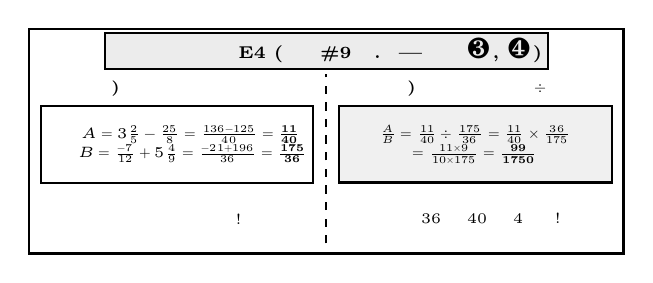
\begin{tikzpicture}[x=0.95cm, y=0.92cm, every node/.style={font=\scriptsize, text=black}]
  \draw[black, line width=0.95pt] (0,0) rectangle (7.95,3.10);
  \node[fill=gray!15, draw=black, line width=0.6pt, inner sep=2pt, font=\fontsize{6.2pt}{7.9pt}\selectfont\bfseries] at (3.975,2.80) {យុទ្ធសាស្ត្របំបែកប្រភាគធំ \en{E4} (លំហាត់ \#9ច ទំ.១២ — ហេតុផល \cnum{3}, \cnum{4})};

  \draw[black, dashed, line width=0.65pt] (3.975,0.14) -- (3.975,2.48);

  \node[font=\fontsize{5.6pt}{7.2pt}\selectfont\bfseries] at (1.98,2.28) {១) គណនាភាគយក និងភាគបែងដាច់គ្នា};
  \draw[black, line width=0.75pt] (0.16,0.98) rectangle (3.80,2.04);
  \node[align=center, font=\fontsize{5.4pt}{7.0pt}\selectfont] at (1.98,1.51) {ភាគយក $A = 3\frac{2}{5}-\frac{25}{8} = \frac{136-125}{40} = \mathbf{\frac{11}{40}}$\\ភាគបែង $B = \frac{-7}{12}+5\frac{4}{9} = \frac{-21+196}{36} = \mathbf{\frac{175}{36}}$};
  \node[font=\fontsize{5.3pt}{6.8pt}\selectfont] at (1.98,0.48) {កុំគណនាលាយឡំក្នុងប្រភាគធំតែមួយ!};

  \node[font=\fontsize{5.6pt}{7.2pt}\selectfont\bfseries] at (5.96,2.28) {២) ប្ដូររបារប្រភាគធំជាសញ្ញា $\div$};
  \draw[black, line width=0.8pt, fill=gray!12] (4.14,0.98) rectangle (7.79,2.04);
  \node[align=center, font=\fontsize{5.4pt}{7.0pt}\selectfont] at (5.965,1.51) {$\frac{A}{B} = \frac{11}{40}\div\frac{175}{36} = \frac{11}{40}\times\frac{36}{175}$\\$= \frac{11\times 9}{10\times 175} = \mathbf{\frac{99}{1750}}$};
  \node[font=\fontsize{5.3pt}{6.8pt}\selectfont] at (5.965,0.48) {សម្រួល $36$ នឹង $40$ នឹង $4$ មុនគុណ!};
\end{tikzpicture}}

% ៤. E5 Diagnostic Cards A-D
\newcommand{\figExitCardsRATPROB}{%
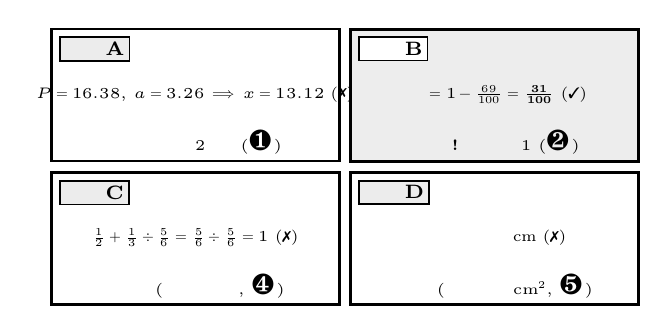
\begin{tikzpicture}[x=0.95cm, y=0.92cm, every node/.style={font=\scriptsize, text=black}]
  \draw[black, line width=0.9pt] (0,1.98) rectangle (3.85,3.80);
  \node[anchor=north west, fill=gray!15, draw=black, line width=0.6pt, inner sep=1.8pt] at (0.10,3.70) {\textbf{ជម្រើស \en{A}}};
  \node[font=\fontsize{5.5pt}{7.1pt}\selectfont] at (1.925,2.90) {$P=16.38,\; a=3.26 \implies x=13.12$ (\ding{55})};
  \node[font=\fontsize{5.4pt}{7.0pt}\selectfont] at (1.925,2.24) {ភ្លេចចែកបរិមាត្រនឹង $2$ ជាមុន (\cnum{1})};

  \draw[black, line width=1.1pt, fill=gray!14] (4.00,1.98) rectangle (7.85,3.80);
  \node[anchor=north west, fill=white, draw=black, line width=0.6pt, inner sep=1.8pt] at (4.10,3.70) {\textbf{ជម្រើស \en{B}}};
  \node[font=\fontsize{5.5pt}{7.1pt}\selectfont] at (5.925,2.90) {សន្សំ $= 1-\frac{69}{100} = \mathbf{\frac{31}{100}}$ (\ding{51})};
  \node[font=\fontsize{5.4pt}{7.0pt}\selectfont] at (5.925,2.24) {\textbf{ត្រឹមត្រូវ!} ដកពីឯកតាពេញ $1$ (\cnum{2})};

  \draw[black, line width=0.9pt] (0,0) rectangle (3.85,1.82);
  \node[anchor=north west, fill=gray!15, draw=black, line width=0.6pt, inner sep=1.8pt] at (0.10,1.72) {\textbf{ជម្រើស \en{C}}};
  \node[font=\fontsize{5.5pt}{7.1pt}\selectfont] at (1.925,0.92) {$\frac{1}{2}+\frac{1}{3}\div\frac{5}{6} = \frac{5}{6}\div\frac{5}{6} = 1$ (\ding{55})};
  \node[font=\fontsize{5.4pt}{7.0pt}\selectfont] at (1.925,0.26) {ខុសអាទិភាព (ត្រូវធ្វើចែកមុនបូក, \cnum{4})};

  \draw[black, line width=0.9pt] (4.00,0) rectangle (7.85,1.82);
  \node[anchor=north west, fill=gray!15, draw=black, line width=0.6pt, inner sep=1.8pt] at (4.10,1.72) {\textbf{ជម្រើស \en{D}}};
  \node[font=\fontsize{5.5pt}{7.1pt}\selectfont] at (5.925,0.92) {ក្រឡាផ្ទៃគិតជាខ្នាត $\unit{cm}$ (\ding{55})};
  \node[font=\fontsize{5.4pt}{7.0pt}\selectfont] at (5.925,0.26) {ខុសខ្នាត (ក្រឡាផ្ទៃគិតជា $\unit{cm}^2$, \cnum{5})};
\end{tikzpicture}}

\begin{document}
\fontsize{10pt}{15.2pt}\selectfont

% -------------------- ក្បាលកិច្ចតែងការ --------------------
\begin{center}
  {\muol\fontsize{11pt}{16pt}\selectfont ព្រះរាជាណាចក្រកម្ពុជា}\\[2pt]
  {\muol\fontsize{10pt}{15pt}\selectfont ជាតិ សាសនា ព្រះមហាក្សត្រ}\\[1pt]
  \khmflourish
\end{center}

\vspace{-24pt}
{\muol\fontsize{9.5pt}{12.5pt}\selectfont
មន្ទីរអប់រំ យុវជន និងកីឡា ខេត្តកំពង់ធំ\\
ការិយាល័យអប់រំ យុវជន និងកីឡា ស្រុកកំពង់ស្វាយ\\
អនុវិទ្យាល័យព្រះក្រសាំង}

\vspace{1pt}
\begin{center}
  {\muol\fontsize{10pt}{14pt}\selectfont កិច្ចតែងការបង្រៀន}
\end{center}
\vspace{0pt}

% -------------------- ព័ត៌មានទូទៅ --------------------
{\renewcommand{\arraystretch}{0.98}
\hspace*{3.1cm}%
\begin{tabular}{@{}l l L{11.0cm}@{}}
  - \hspace{0.35cm} មុខវិជ្ជា & : & គណិតវិទ្យា ថ្នាក់ទី៨ (ពីជគណិត) \\
  - \hspace{0.35cm} ចំណងជើងមេរៀន & : & មេរៀនទី១៖ ចំនួនសនិទាន \\
  - \hspace{0.35cm} ចំណងជើងរង & : & ៦. ចំណោទ និងសំយោគមេរៀនទី១ (សៀវភៅពុម្ព ទំ.១០–១២) \\
  - \hspace{0.35cm} រយៈពេល & : & ១ ម៉ោងសិក្សា (៥០ នាទី) \\
  - \hspace{0.35cm} បង្រៀនដោយ & : & ហុក ប៊ុនថែន \\
  - \hspace{0.35cm} កាលបរិច្ឆេទ & : & ថ្ងៃចន្ទ ទី២៣ ខែវិច្ឆិកា ឆ្នាំ២០២៦ \\
\end{tabular}

\vspace{2pt}

% -------------------- I. វត្ថុបំណង --------------------
\textbf{I.} {\muol វត្ថុបំណង}\\[1pt]
\hspace*{0.55cm}%
\begin{tabular}{@{}l l L{14.2cm}@{}}
  \wcirc \hspace{0.25cm} វិជ្ជាសម្បទា & : & សិស្សប្រាប់ដំណាក់កាលទាំង ៤ នៃការដោះស្រាយចំណោទចំនួនសនិទាន (គំនូសតាង/តាងអញ្ញាត ទំនាក់ទំនង គណនា និងផ្ទៀងផ្ទាត់) និងលំដាប់ប្រមាណវិធីទាំង ៤ បានត្រឹមត្រូវតាមសៀវភៅគោល (ទំ.១០–១២) ។ \\
  \wcirc \hspace{0.25cm} បំណិនសម្បទា & : & សិស្សដោះស្រាយចំណោទធរណីមាត្រ (បរិមាត្រ-ក្រឡាផ្ទៃ) ចំណោទដ្យាក្រាមផ្លិតប្រាក់សន្សំ និងកន្សោមប្រភាគជាប់ប្រភាគលើសន្លឹកកិច្ចការដោយដៃបានត្រឹមត្រូវ ។ \\
  \wcirc \hspace{0.25cm} ចរិយាសម្បទា & : & សិស្សមានទម្លាប់គូសគំនូសប្លង់មុនគណនា ផ្ទៀងផ្ទាត់ខ្នាត និងយល់ឃើញអត្ថប្រយោជន៍នៃចំនួនសនិទានក្នុងការគ្រប់គ្រងថវិកាគ្រួសារប្រចាំថ្ងៃ ។ \\
\end{tabular}

\vspace{2pt}

% -------------------- II. សម្ភារៈឧបទេស --------------------
\textbf{II.} {\muol សម្ភារៈឧបទេស}\\[1pt]
\hspace*{0.55cm}$\bullet$ \hspace{0.35cm} សៀវភៅសិក្សាគោលគណិតវិទ្យាថ្នាក់ទី៨ (ទំ.១០–១២) ក្ដារខៀន ដីស បន្ទាត់ និងសន្លឹកកិច្ចការសិស្ស ស-ខ្មៅ (\en{Worksheet\_RAT\_PROB} ទំព័រ ១–២ គ្មានស្លាយ \en{LCD} គ្មានម៉ាស៊ីនគិតលេខ)

\vspace{2pt}

% -------------------- III. វិធីសាស្រ្តបង្រៀន --------------------
\textbf{III.} {\muol វិធីសាស្រ្តបង្រៀន}\\[1pt]
\hspace*{0.45cm}%
\begin{tabular}{@{}l l L{14.85cm}@{}}
  $\bullet$ \hspace{0.25cm} គោលវិធី & : & សិស្សមជ្ឈមណ្ឌល (បង្រៀនតាមសន្លឹកកិច្ចការគំនូសប្លង់ស៊ើបអង្កេតជាដៃគូ និងក្ដារខៀន គ្មាន \en{LCD}) \\
  $\bullet$ \hspace{0.25cm} យុទ្ធវិធីបង្រៀន & : & គំរូ \en{5Es} រួមបញ្ចូលគំនូសប្លង់ ៤ ជំហានបែបសិង្ហបុរី \en{(POE 1)}, ដ្យាក្រាមផ្លិត \en{(POE 2)} និងការបំបែកប្រភាគធំ \\
\end{tabular}
}

\vspace{2pt}

% -------------------- IV. ដំណើរការបង្រៀន --------------------
\textbf{IV.} {\muol ដំណើរការបង្រៀន}

\vspace{1pt}

\renewcommand{\arraystretch}{1.15}
\begin{longtable}{|L{5.50cm}|L{7.90cm}|L{4.80cm}|}
\hline
\rowcolor{headgray}
\multicolumn{1}{|c|}{\muol សកម្មភាពគ្រូ} &
\multicolumn{1}{c|}{\muol ខ្លឹមសារមេរៀន} &
\multicolumn{1}{c|}{\muol សកម្មភាពសិស្ស} \\
\hline
\endfirsthead

\hline
\rowcolor{headgray}
\multicolumn{1}{|c|}{\muol សកម្មភាពគ្រូ} &
\multicolumn{1}{c|}{\muol ខ្លឹមសារមេរៀន} &
\multicolumn{1}{c|}{\muol សកម្មភាពសិស្ស} \\
\hline
\endhead

\hline
\endfoot

\hline
\endlastfoot

% ==================== ជំហានទី១ (2min) ====================
\stepheader{ជំហានទី១ \enbf{(}រដ្ឋបាលថ្នាក់\enbf{)}}
$\bullet$ ពិនិត្យអវត្តមាន អនាម័យ និងសណ្ដាប់ធ្នាប់ថ្នាក់រៀន \timenote{(2 min)}\par\vspace{2pt}
$\bullet$ ចែក \textbf{សន្លឹកកិច្ចការសិស្ស (\en{Worksheet\_RAT\_PROB})} ម្នាក់ ១ សន្លឹក (ផ្កាប់ទុកសិន)
&
$\bullet$ រដ្ឋបាលថ្នាក់ និងការរៀបចំដៃគូសិក្សា (២ នាក់ក្នុង ១ តុ)\par\vspace{2pt}
$\bullet$ សន្លឹកកិច្ចការសិស្ស ស-ខ្មៅ ២ ទំព័រ សម្រាប់បំពេញតាមជំហានមេរៀន
&
$\circ$ ប្រធានថ្នាក់រាយការណ៍អវត្តមាន\par\vspace{2pt}
$\circ$ ទទួលសន្លឹកកិច្ចការ ដាក់ផ្កាប់លើតុ \\[5pt]
\hline

% ==================== ជំហានទី២ (9min: <=3 + 3 + E1 3) ====================
\stepheader{ជំហានទី២ \enbf{(}កិច្ចការផ្ទះ \enbf{+} ទំនាក់ទំនងមេរៀនថ្មី\enbf{)}}
\timenote{កំណែកិច្ចការផ្ទះ ($\le 3\unit{min}$)}\par\vspace{2pt}
$\bullet$ ហៅសិស្ស ២ នាក់ឡើងកែកិច្ចការផ្ទះចំណុច ៥ លើក្ដារខៀន
&
\textbf{១. កំណែកិច្ចការផ្ទះ (ប្រមាណវិធីចែកចំនួនសនិទាន)៖}\par\vspace{2.5pt}
$\bullet$ \textbf{១ក)} $-\dfrac{15}{28}\div\dfrac{5}{-14} = \left(-\dfrac{15}{28}\right)\times\left(-\dfrac{14}{5}\right) = \dfrac{3}{2}$\par\vspace{2.5pt}
$\bullet$ \textbf{១ខ)} $\left(\dfrac{1}{2}+\dfrac{1}{3}\right)\div\left(\dfrac{5}{8}-\dfrac{1}{4}\right) = \dfrac{5}{6}\div\dfrac{3}{8} = \dfrac{20}{9}$\par\vspace{2.5pt}
$\bullet$ \textbf{២)} កន្លះបរិមាត្រចតុកោណកែង $p = 16.38\div 2 = 8.19\unit{cm}$
&
$\circ$ តំណាងសិស្សឡើងកែលើក្ដារខៀន\par\vspace{2pt}
$\circ$ ផ្ទៀងផ្ទាត់ និងកែតម្រូវចូលសៀវភៅ \\[5pt]

\timenote{រំលឹកមេរៀនទាក់ទង (3 min)}\par\vspace{2pt}
$\bullet$ សួររំលឹករូបមន្តបរិមាត្រ-ក្រឡាផ្ទៃចតុកោណកែង និងលំដាប់ប្រមាណវិធីទាំង ៤ នៃចំនួនសនិទាន
&
\textbf{២. រំលឹករូបមន្តធរណីមាត្រ និងអាទិភាពប្រមាណវិធី៖}\par\vspace{2pt}
$\bullet$ ចតុកោណកែងជ្រុង $a, b$៖ $P = 2(a+b)$, កន្លះបរិមាត្រ $p = a+b$, ក្រឡាផ្ទៃ $S = a\times b$
&
$\circ$ ឆ្លើយផ្ទាល់មាត់ពីរូបមន្ត $P, p, S$ \\[3pt]

$\bullet$ សួរបញ្ជាក់ពីអាទិភាពប្រមាណវិធី៖ «បើមានវង់ក្រចក បូក ដក គុណ និងចែក តើធ្វើមួយណាមុន?»
&
$\bullet$ អាទិភាព៖ វង់ក្រចក $\to$ គុណ/ចែក (ឆ្វេងទៅស្ដាំ) $\to$ បូក/ដក
&
$\circ$ ឆ្លើយផ្ទាល់មាត់តាមលំដាប់អាទិភាព \\[3pt]

\fiveE{E1 - Engage} \timenote{(3 min)}\par\vspace{2pt}
$\bullet$ ឱ្យសិស្សផ្ងារសន្លឹកកិច្ចការទំព័រទី១ អានបេសកកម្ម \en{E1} (\textbf{លំហាត់ \#11 ទំ.១២})៖ «តើពិតឬទេដែលថា $\frac{13}{4}+\frac{13}{9}$ ស្មើនឹង $\frac{13}{4}\times\frac{13}{9}$ បេះបិទ?»
&
\textbf{៣. បេសកកម្ម \en{E1} — គូប្រភាគអច្ឆរិយៈ (\#11 ទំ.១២)៖}\par\vspace{2pt}
$\bullet$ ផលបូក $=\dfrac{117+52}{36}=\mathbf{\dfrac{169}{36}}$ និងផលគុណ $=\dfrac{13\times 13}{4\times 9}=\mathbf{\dfrac{169}{36}}$ (ពិត!)\par\vspace{2pt}
$\bullet$ ភ្ជាប់ចូលមេរៀនថ្មី៖ \textbf{៦. ចំណោទ និងសំយោគមេរៀនទី១ (ទំ.១០–១២)}
&
$\circ$ ភ្ញាក់ផ្អើលពេលគណនាឃើញ $\frac{169}{36}$ ស្មើគ្នាទាំងផលបូក និងផលគុណ! \\[3pt]

& \cfig{\figEngageRATPROB} & \\[3pt]
\hline

% ==================== ជំហានទី៣ (17min: E2 11 + E3 6) ====================
\stepheader{ជំហានទី៣ \enbf{(}ខ្លឹមសារមេរៀនថ្មី\enbf{)}}
\fiveE{E2 - Explore} \timenote{(11 min)}\par\vspace{2pt}
$\bullet$ សរសេរចំណងជើងមេរៀនលើក្ដារខៀន និងណែនាំ \textbf{សកម្មភាពទី១ (\en{POE 1} — ចំណោទចតុកោណកែង ទំ.១០–១១)}៖\par\vspace{2pt}
\hspace*{0.3em}-- \textbf{អន្ទាក់ទស្សន៍ទាយ៖} «បើ $P=16.38\unit{cm}$ និងទទឹង $3.26\unit{cm}$ តើបណ្ដោយ $x = 16.38-3.26$ មែនឬទេ?»
&
\textbf{៦. ចំណោទ (សៀវភៅពុម្ព ទំ.១០–១១) — \en{POE 1}៖}\par\vspace{2pt}
$\bullet$ \textbf{ក) កន្លះបរិមាត្រ $p$៖} $p = 16.38\div 2 = \graybox{$8.19\unit{cm}$}$ (មិនមែន $16.38$ ទេ!)\par\vspace{2pt}
$\bullet$ \textbf{ខ) ជ្រុងមួយទៀត $x$៖} $x + 3.26 = 8.19 \implies x = 8.19 - 3.26 = \graybox{$4.93\unit{cm}$}$
&
$\circ$ កត់សម្គាល់អន្ទាក់ភ្លេចចែកបរិមាត្រនឹង $2$ រួចគណនា $p$ និង $x$ ជាដៃគូ \\[3pt]

$\bullet$ ឱ្យដៃគូគណនា \textbf{សំណួរ គ} (ផ្ទៃក្រឡា $S$) ដោយដៃ និងផ្ទៀងផ្ទាត់បរិមាត្រឡើងវិញ
&
$\bullet$ \textbf{គ) ផ្ទៃក្រឡា $S$៖} $S = 3.26\times 4.93 = \graybox{$16.0718\unit{cm}^2$}$\par\vspace{2pt}
$\bullet$ \textbf{ផ្ទៀងផ្ទាត់៖} $2\times(3.26 + 4.93) = 2\times 8.19 = 16.38\unit{cm}$ (\ding{51})
&
$\circ$ គុណទសភាគដោយដៃ (កាត់ក្បៀស $4$ ខ្ទង់) និងដាក់ខ្នាត $\unit{cm}^2$ \\[3pt]

$\bullet$ ណែនាំ \textbf{សកម្មភាពទី២ (\en{POE 2} — ដ្យាក្រាមផ្លិតប្រាក់ខែ \#14 ទំ.១២)}៖ ម្ហូប $\frac{1}{2}$, ធ្វើដំណើរ $\frac{1}{20}$, កំសាន្ត $\frac{1}{10}$, ទឹក-ភ្លើង $\frac{1}{25}$ — រកប្រភាគប្រាក់សន្សំ
&
\textbf{ចំណោទដ្យាក្រាមផ្លិត (ទំ.១២ \#14) — \en{POE 2}៖}\par\vspace{2pt}
$\bullet$ តម្រូវភាគបែងរួម $100$៖ ចំណាយសរុប $=\dfrac{1}{2}+\dfrac{1}{20}+\dfrac{1}{10}+\dfrac{1}{25} = \dfrac{50+5+10+4}{100} = \dfrac{69}{100}$\par\vspace{2pt}
$\bullet$ \textbf{ប្រភាគប្រាក់សន្សំ៖} $1 - \dfrac{69}{100} = \dfrac{100-69}{100} = \graybox{$\dfrac{31}{100}$}$
&
$\circ$ បូកប្រភាគចំណាយទាំង ៤ រួចយកឯកតាពេញ $1$ ដកចេញឃើញ $\frac{31}{100}$! \\[3pt]

& \cfig{\figModelsRATPROB} & \\[3pt]

\fiveE{E3 - Explain} \timenote{(6 min)}\par\vspace{2pt}
$\bullet$ ហៅតំណាងដៃគូសង្ខេប \textbf{ដំណាក់កាលទាំង ៤ នៃការដោះស្រាយចំណោទចំនួនសនិទាន} លើក្ដារខៀន
&
\textbf{សំយោគវិធីដោះស្រាយចំណោទ ៤ ជំហាន និងធនាគារហេតុផល (\cnum{1}--\cnum{5})៖}\par\vspace{2pt}
$\bullet$ \textbf{៤ ជំហាន៖} (១) គូសប្លង់/តាងអញ្ញាត $\to$ (២) សរសេរទំនាក់ទំនង $\to$ (៣) គណនាដោយដៃ $\to$ (៤) ផ្ទៀងផ្ទាត់ចម្លើយ និងខ្នាត
&
$\circ$ បំពេញជំហានទាំង ៤ ក្នុងប្រអប់សំយោគលើសន្លឹកកិច្ចការ \\[3pt]

$\bullet$ សង្ខេបធនាគារហេតុផល \cnum{1}--\cnum{3} សម្រាប់ចំណោទធរណីមាត្រ ឯកតាពេញ $1$ និងប្រភាគធំ
&
\cnum{1} គំនូសប្លង់ចតុកោណកែង៖ កន្លះបរិមាត្រ $p = P\div 2 = a+b$ និងផ្ទៃក្រឡា $S = a\cdot b$ ។\par\vspace{1.5pt}
\cnum{2} ដ្យាក្រាមផ្លិត/ឯកតាពេញ $1$៖ ផ្នែកនៅសល់ $= 1 - (\text{ផលបូកប្រភាគផ្នែកស្គាល់})$ ។\par\vspace{1.5pt}
\cnum{3} ប្រភាគធំ $\frac{A}{B}$៖ គណនាភាគយក $A$ ដាច់ និងភាគបែង $B$ ដាច់ រួចប្ដូរជា $A\div B$ ។
&
$\circ$ ផ្ទៀងផ្ទាត់ហេតុផល \cnum{1}--\cnum{3} លើសន្លឹកកិច្ចការ \\[3pt]

$\bullet$ បញ្ជាក់ហេតុផល \cnum{4}--\cnum{5} សម្រាប់អាទិភាពប្រមាណវិធី និងការផ្ទៀងផ្ទាត់ខ្នាត
&
\cnum{4} អាទិភាពប្រមាណវិធី៖ វង់ក្រចក $\to$ គុណ/ចែក $\to$ បូក/ដក (ប្រើលក្ខណៈបំបែកបើមានកត្តារួម) ។\par\vspace{1.5pt}
\cnum{5} ផ្ទៀងផ្ទាត់សមហេតុផល និងខ្នាត៖ ប្រវែង ($\unit{cm}$), ក្រឡាផ្ទៃ ($\unit{cm}^2$), ផលបូកប្រភាគស្មើ $1$ ។
&
$\circ$ ធ្វើលំហាត់ត្រួតពិនិត្យរហ័សនៅបាតទំព័រទី១ \\[3pt]
\hline

% ==================== ជំហានទី៤ (20min: E4 10 + E5 10) ====================
\stepheader{ជំហានទី៤ \enbf{(}ពង្រឹង និងពង្រីកចំណេះដឹង\enbf{)}}
\fiveE{E4 - Elaborate} \timenote{(10 min)}\par\vspace{2pt}
$\bullet$ ឱ្យសិស្សបើកសន្លឹកកិច្ចការទំព័រទី២ (ផ្នែកទី៣) បំបែក \textbf{លំហាត់ប្រភាគធំ \#9ច} និង \textbf{\#10គ} (ទំ.១២)
&
\textbf{១. សំយោគកន្សោមប្រភាគធំ និងលក្ខណៈបំបែក (សៀវភៅពុម្ព ទំ.១២)៖}\par\vspace{2.5pt}
$\bullet$ \textbf{\#9ច (ទំ.១២)៖} $\dfrac{3\frac{2}{5}-\frac{25}{8}}{\frac{-7}{12}+5\frac{4}{9}} = \dfrac{11}{40}\div\dfrac{175}{36} = \dfrac{11}{40}\times\dfrac{36}{175} = \graybox{$\dfrac{99}{1750}$} \quad (\text{\cnum{3}})$\par\vspace{3pt}
$\bullet$ \textbf{\#10គ (ទំ.១២)៖} $\left(-\dfrac{11}{13}+\dfrac{17}{16}\right)\cdot\dfrac{26}{22} = \dfrac{45}{208}\cdot\dfrac{13}{11} = \graybox{$\dfrac{45}{176}$} \quad (\text{\cnum{4}})$
&
$\circ$ គណនាភាគយក-ភាគបែងដាច់គ្នា រួចសម្រួលខ្វែងដោយដៃ \\[3pt]

$\bullet$ ដឹកនាំការបង្ហាញលក្ខណៈបំបែកចំពោះវិធីដក (\textbf{\#12 ទំ.១២}) និងសំណួរ \en{EIA Looking-Back}
&
$\bullet$ \textbf{\#12 (ទំ.១២)៖} $\dfrac{a}{b}\left(\dfrac{c}{d}-\dfrac{e}{f}\right) = \dfrac{a}{b}\left[\dfrac{c}{d}+\left(-\dfrac{e}{f}\right)\right] = \dfrac{a}{b}\cdot\dfrac{c}{d} - \dfrac{a}{b}\cdot\dfrac{e}{f}$\par\vspace{3pt}
&
$\circ$ បកស្រាយភ្ជាប់វិធីដកទៅនឹងវិធីបូកចំនួនផ្ទុយ \\[4pt]

& \cfig{\figComplexFracRATPROB} & \\[3pt]

\fiveE{E5 - Evaluate} \timenote{(10 min)}\par\vspace{2pt}
$\bullet$ ឱ្យសិស្សធ្វើចំណោទអនុវត្តន៍ជាដៃគូលើសន្លឹកកិច្ចការ (រងបន្លែ $P=12.4\unit{m}$, ទទឹង $2.5\unit{m}$) រួចផ្ទៀងផ្ទាត់ (\en{Pause-Review})
&
\textbf{២. ចំណោទអនុវត្តន៍ និងការផ្ទៀងផ្ទាត់អសមភាព (\#13 ទំ.១២)៖}\par\vspace{2pt}
$\bullet$ \textbf{ចំណោទរងបន្លែ៖} $p = 12.4\div 2 = \mathbf{6.2\unit{m}}$ \;;\; បណ្ដោយ $x = 6.2 - 2.5 = \mathbf{3.7\unit{m}}$ \;;\; ក្រឡាផ្ទៃ $S = 2.5\times 3.7 = \mathbf{9.25\unit{m}^2}$
&
$\circ$ ដោះស្រាយតាម ៤ ជំហាន និងផ្ទៀងផ្ទាត់ខ្នាតជាដៃគូ \\[4pt]

$\bullet$ បន្តផ្ទៀងផ្ទាត់អសមភាព \#13 (ទំ.១២) និងបិទបញ្ចប់បេសកកម្ម \en{E1}
&
$\bullet$ \textbf{\#13 (ទំ.១២)៖} បើ $\frac{1}{3}<\frac{1}{2}$ បូកនឹង $\frac{1}{6}$ បាន $\frac{1}{2}<\frac{2}{3}$ (ពិត!) \;\en{|}\; \textbf{បិទ \en{E1}៖} $\mathbf{\dfrac{169}{36}}$
&
$\circ$ ផ្ទៀងផ្ទាត់អសមភាព និងបិទបញ្ចប់បេសកកម្ម \en{E1} \\[4pt]

$\bullet$ វាយតម្លៃរហ័ស \textbf{៦០ វិនាទី}៖ ឱ្យសិស្សគូសវង់ជម្រើសត្រឹមត្រូវក្នុងប្រអប់ \en{A--D} និងបំពេញសំបុត្រចេញ
&
\textbf{៣. វិនិច្ឆ័យកំហុសរហ័ស (\en{A--D})៖} ចម្លើយត្រឹមត្រូវគឺ \graybox{\textbf{ជម្រើស \en{B}}} ($\frac{31}{100}$) ។\par\vspace{2pt}
(\en{A} ភ្លេចចែកបរិមាត្រនឹង $2$; \en{C} ខុសអាទិភាពបូកមុនចែក; \en{D} ខុសខ្នាតក្រឡាផ្ទៃ)
&
$\circ$ គូសវង់ជម្រើស \en{B} និងបំពេញសំបុត្រចេញមុនបញ្ចប់ម៉ោង \\[3pt]

& \cfig{\figExitCardsRATPROB} & \\[3pt]
\hline

% ==================== ជំហានទី៥ (<=2min) ====================
\stepheader{ជំហានទី៥ \enbf{(}កិច្ចការផ្ទះ \enbf{+} បណ្ដាំផ្ញើ\enbf{)}}
\timenote{ចំណាយពេលឱ្យតិចបំផុតកុំឱ្យលើស 2 min}\par\vspace{2pt}
$\bullet$ ណែនាំកិច្ចការផ្ទះសំយោគ និងបុរេសិក្សាគុណកត្តាដូចគ្នា ដើម្បីភ្ជាប់ចូល \textbf{មេរៀនទី២៖ ស្វ័យគុណ (២.១ សញ្ញាណស្វ័យគុណ ទំ.១៣–១៤)}
&
\centerline{\muol កិច្ចការផ្ទះ}\par\vspace{2pt}
$\bullet$ \textbf{លំហាត់ ១ (បុរេសិក្សាភ្ជាប់មេរៀនទី២)៖} គណនាផលគុណកត្តាដូចគ្នា៖\par\vspace{2pt}
\hspace*{0.3cm}ក) $(-4)\times(-4)$ និង $(-4)\times(-4)\times(-4)$\par\vspace{2pt}
\hspace*{0.3cm}ខ) $\left(\dfrac{2}{3}\right)\times\left(\dfrac{2}{3}\right)$\par\vspace{2pt}
$\bullet$ \textbf{លំហាត់ ២ (សំយោគមេរៀនទី១)៖} គ្រួសារមួយចំណាយលើម្ហូប $\frac{2}{5}$, សិក្សា $\frac{1}{4}$ និងទឹក-ភ្លើង $\frac{1}{10}$ ។ រកប្រភាគប្រាក់សន្សំ ។\par\vspace{2pt}
$\bullet$ \textbf{បណ្ដាំផ្ញើ៖} អានមុន \textbf{មេរៀនទី២៖ ស្វ័យគុណ (២.១ សញ្ញាណស្វ័យគុណ ទំ.១៣–១៤)} ។
&
$\circ$ កត់ត្រាកិច្ចការផ្ទះ និងត្រៀមចូលមេរៀនទី២ នៅម៉ោងបន្ទាប់ \\[3pt]
\end{longtable}

% -------------------- កាលបរិច្ឆេទ និងហត្ថលេខា --------------------
\vspace{2pt}
\hfill
\begin{minipage}{9.8cm}
  {\centering
    ថ្ងៃចន្ទ ១៤កើត ខែកត្តិក ឆ្នាំមមី អដ្ឋស័ក ពុទ្ធសករាជ ២៥៧០\\[2pt]
    ត្រូវនឹងថ្ងៃទី២៣ ខែវិច្ឆិកា ឆ្នាំ២០២៦\\[3pt]
    {\muol គ្រូបង្រៀន}\par}
  \vspace{32pt}
  \hfill{\muol ហុក ប៊ុនថែន}\hspace*{1.4cm}
\end{minipage}

\end{document}
